\documentclass{beamer}
\usefonttheme[onlymath]{serif}

\usepackage[utf8]{inputenc}
\usepackage[T1]{fontenc}
\usepackage{lmodern}
\usepackage[francais]{babel}

% For table
\usepackage{booktabs} % To thicken table lines
\usepackage{multirow}
\usepackage{amsmath}

\usepackage[group-separator={,}]{siunitx}

  %for tikz figure
\usepackage{tikz}
\usetikzlibrary{decorations.pathreplacing}
\usetikzlibrary{fadings}
\usetikzlibrary{positioning} %for lstm
\usetikzlibrary{shapes, backgrounds}
\usetikzlibrary{arrows}
\usetikzlibrary{chains}
\tikzstyle{line} = [draw, -latex']
\usepackage{adjustbox}

\usepackage{pgfplots}
\usepackage{pgfplotstable}

\definecolor{color3}{rgb}{0,0.7,0.3}
\definecolor{color1}{rgb}{0,0.1,0.8}
\definecolor{color2}{rgb}{0.9,0.0,0}

\graphicspath{{img/}}


\mode<presentation> {
	\usetheme{ulaval}
	\setbeamercovered{invisible}
}

\logo{
	
\includegraphics[height=0.65cm, keepaspectratio]{graal.pdf}\hspace{.2cm}\vspace{.85\paperheight}}


\title{Reproductibilité en apprentissage automatique}
%\subtitle[]{}

\author[D. Beauchemin]{David Beauchemin}
\institute[Université Laval]
{
	Département d'informatique et de génie logiciel, \\
	Université Laval\\
	\medskip
	{\emph{david.beauchemin.5@ulaval.ca}}
}
\date{30 octobre 2020}

\AtBeginSection[]
{
	\begin{frame}<beamer>
		\frametitle{Plan}
		\tableofcontents[currentsection]
	\end{frame}
}

\begin{document}
	
	
	\begin{frame}[label=titre, plain]
		\titlepage
		\begin{center}
			
\includegraphics[height=1cm]{graal}
			
\includegraphics[height=1cm]{UL_P}
		\end{center}
	\end{frame}

	\begin{frame}{Objectifs de la présentation}
		\begin{itemize}
			\item Sensibiliser sur les enjeux de la reproductibilité.
			\item Inciter l'intégration des solutions permettant une meilleure reproductibilité dans vos solutions d'affaires ou académiques.
		\end{itemize}
	\end{frame}

	\begin{frame}{Mes qualifications}
		\begin{itemize}
			\item Introduit (informellement) à la recherche reproductible en 2016 (RMarkdown et Git).
			\item Participation à REPROLANG, visant la reproductibilité d'articles scientifiques ayant mené à la publication d'un article en 2019.
			\item Développement en cours de solution d'intégration facilitant la reproductibilité (Poutyne, MLFlow callback).
			\item Candidat au doctorat en informatique en apprentissage automatique.
			\item Membre fondateur de Baseline.
		\end{itemize}
	\end{frame}
	
	\section{Introduction}
	\begin{frame}{C'est quoi la reproductibilité ?}
		La reproductibilité est le principe qu'on ne peut tirer de conclusions que d'un événement bien décrit, qui est apparu plusieurs fois, provoqué par des \textbf{personnes différentes}.
		
		Toutefois, on utilise souvent ce terme pour spécifiquement désigné la \textbf{réplicabilité}. Soit la réplication (reproduction) des résultats d'un articles dans des environnements pas toujours différents \cite{replicationvsreproductiblity, pineau2020improving}.
	\end{frame}

	\begin{frame}{En somme}
		\begin{itemize}
			\item Être capable de répliquer les résultats d'un article,
			\item à partir du même jeux de données ou un jeux de données différents (mais proche),
			\item en utilisant la procédure d'entrainement de l'article et
			\item en utilisant le code du projet.
		\end{itemize}
	\end{frame}

	\begin{frame}{Pourquoi s'y intéressé?}
		\begin{itemize}
			\item $70$~\% des chercheurs en science on échoué dans leur tentative de reproduire un article d'un autre chercheur,
			\item ~$50$~\% n'on pas réussit à reproduire leur \textbf{propre} expérimentation \cite{baker500ScientistsLift2016}.
		\end{itemize}
	\end{frame}

	\begin{frame}{Pourquoi s'y intéressé?}
		L'informatique ne fais pas exception à cela malgré la simplicité (théorique) de réplication des résultats. Selon une étude, sur 255 articles près de $40$~\% n'était pas réplicable \cite{raff2019step}.
	\end{frame}

	\begin{frame}{Pourquoi s'y intéressé?}
		La réplicabilité du code et d'un article facilite la réutilisation pour d'autres projets de recherche \textbf{et} le transfert vers l'industrie. 
	\end{frame}
	
	\section{Les barrières à la réplicabilité}
		\begin{frame}
			\begin{figure}
				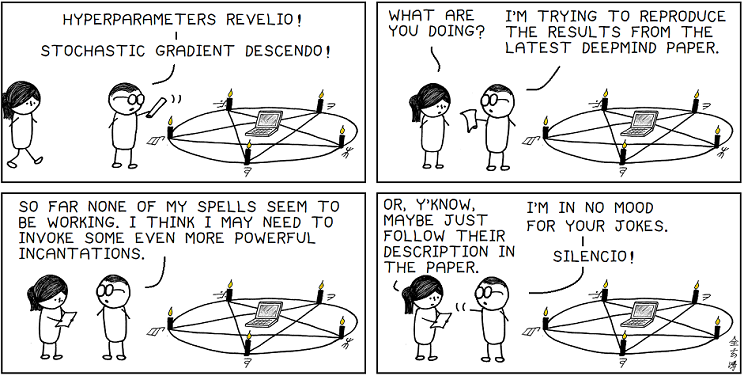
\includegraphics[scale=0.5]{muggle_problems.png}
				\caption{From Abstruse Goose \url{https://abstrusegoose.com/588}}
			\end{figure}
		\end{frame}
	
		\begin{frame}
			\begin{itemize}
				\item Non disponibilité du jeux de données,
				\item Mauvaise spécification ou sous-spécification du modèle ou de la procédure de formation,
				\item Manque de disponibilité du code nécessaire pour exécuter les expériences, ou erreurs dans le code,
				\item Configuration du modèle déficiente \cite{pineau2020improving}\footnote{Liste sélective de ceux présenté dans l'article.}.
			\end{itemize}
		\end{frame}
	
	\section{La reproductibilité jusqu'où?}
	
	\section{La suite}
	
	
	\begin{frame}[t, allowframebreaks]
		\frametitle{References}
		\bibliographystyle{apalike}
		\bibliography{RAA}
	\end{frame}
	
\end{document}